% !TEX TS-program = pdflatex
% !TEX encoding = UTF-8 Unicode

\documentclass[a4paper, titlepage=false, parskip=full-, 10pt]{scrartcl}

\usepackage[utf8]{inputenc}
\usepackage[T1]{fontenc}
\usepackage[english, ngerman]{babel}
\usepackage{babelbib}
\usepackage{hyperref}
\usepackage{listings}
\usepackage{framed}
\usepackage{color}
\usepackage{graphicx}
\usepackage[normalem]{ulem}
\usepackage{cancel}
\usepackage{array}
\usepackage{amsmath}
\usepackage{amssymb}
\usepackage{amsthm}
\usepackage{algorithm}
\usepackage{algorithmic}
\usepackage{geometry}
\usepackage{subfigure}
\geometry{a4paper, top=20mm, left=35mm, right=25mm, bottom=40mm}

\newcounter{tasknbr}
\setcounter{tasknbr}{1}
\newenvironment{task}[1]{{\bf Aufgabe \arabic {tasknbr}\stepcounter{tasknbr}} (#1):\begin{enumerate}}{\end{enumerate}}
\newcommand{\subtask}[1]{\item[#1)]}

% Listings -----------------------------------------------------------------------------
\definecolor{red}{rgb}{.8,.1,.2}
\definecolor{blue}{rgb}{.2,.3,.7}
\definecolor{lightyellow}{rgb}{1.,1.,.97}
\definecolor{gray}{rgb}{.7,.7,.7}
\definecolor{darkgreen}{rgb}{0,.5,.1}
\definecolor{darkyellow}{rgb}{1.,.7,.3}
\lstloadlanguages{C++,[Objective]C,Java}
\lstset{
escapeinside={§§}{§§},
basicstyle=\ttfamily\footnotesize\mdseries,
columns=fullflexible,
keywordstyle=\bfseries\color{blue},
commentstyle=\color{darkgreen},      
stringstyle=\color{red},
numbers=left,
numberstyle=\ttfamily\scriptsize\color{gray},
breaklines=true,
showstringspaces=false,
tabsize=4,
captionpos=b,
float=htb,
frame=tb,
frameshape={RYR}{y}{y}{RYR},
rulecolor=\color{black},
xleftmargin=15pt,
xrightmargin=4pt,
aboveskip=\bigskipamount,
belowskip=\bigskipamount,
backgroundcolor=\color{lightyellow},
extendedchars=true,
belowcaptionskip=15pt}

%% Enter current values here: %%
\newcommand{\lecture}{Robotik WS15/16}
\newcommand{\tutor}{}
\newcommand{\assignmentnbr}{10}
\newcommand{\students}{Julius Auer, Thomas Tegethoff}
%%-------------------------------------%%

\begin{document}  
{\small \textsl{\lecture \hfill \tutor}}
\hrule
\begin{center}
\textbf{Übungsblatt \assignmentnbr}\\
[\bigskipamount]
{\small \students}
\end{center}
\hrule

\begin{task}{Voronoi-Diagramme}
\item[]
Letztes Semester habe ich bereits für eine andere Lehrveranstaltung (Algorithmische Geometrie) Fortune's Sweep implementiert. Genau genommen haben wir dort den Algo nur theoretisch behandelt - Prof. Alt hielt eine Implementierung im Rahmen des Übungsbetriebs für zu aufwändig ;)\\
Ich hatte aber trotzdem Lust dazu, was sich nun auszahlt :)

Der Code ist diesmal in Java. Die Implementierung benötigt eine Anzahl Hilfsklassen (Kreise, Strahlen, Strecken, etc.) weshalb ich die gesamte Codebasis aus Algorithmische Geometrie mit einreichen muss. Solltet Ihr den Code lesen wollen müsst Ihr deshalb etwas suchen, am besten in \emph{geometry/algorithms/FortunesSweep}. Der Code ist mit im Jar.

Das abgegebene Jar ist ausführbar (erfordert Java 7) und visualisiert Fortune's Sweep für 80 zufällig generierte Punkte. Für Keyboard-Controls siehe stdout.

Für zehn zufällige Punkte zeigt Abbildung \ref{fig:1-1} die ersten vier Schritte des Algos und Abbildung \ref{fig:1-2} die letzten vier.

Die Plots sollten einigermaßen selbst-erklärend sein - ungewöhnlich sind vielleicht nur die Cyan-farbenen Linien, die für jedes Parabelsegment den Punkt visualisieren, der die zugehörige Parabel erzeugt hat. Man sieht so auch, wie viele Segmente einer Parabel noch ''im Rennen'' sind.

Es ist anzumerken, dass die Parabelsegmente hier nicht in einem Baum (sondern nur in einer Liste) gespeichert werden. Dadurch wird die worst-case Laufzeit quadratisch! Da hier die Visualisierung im Vordergrund stand und die Implementierung des Baums doch recht aufwändig gewesen wäre, haben wir das in Kauf genommen.

\begin{figure}[!htpb]
\centering
\subfigure[Schritt 1]{
  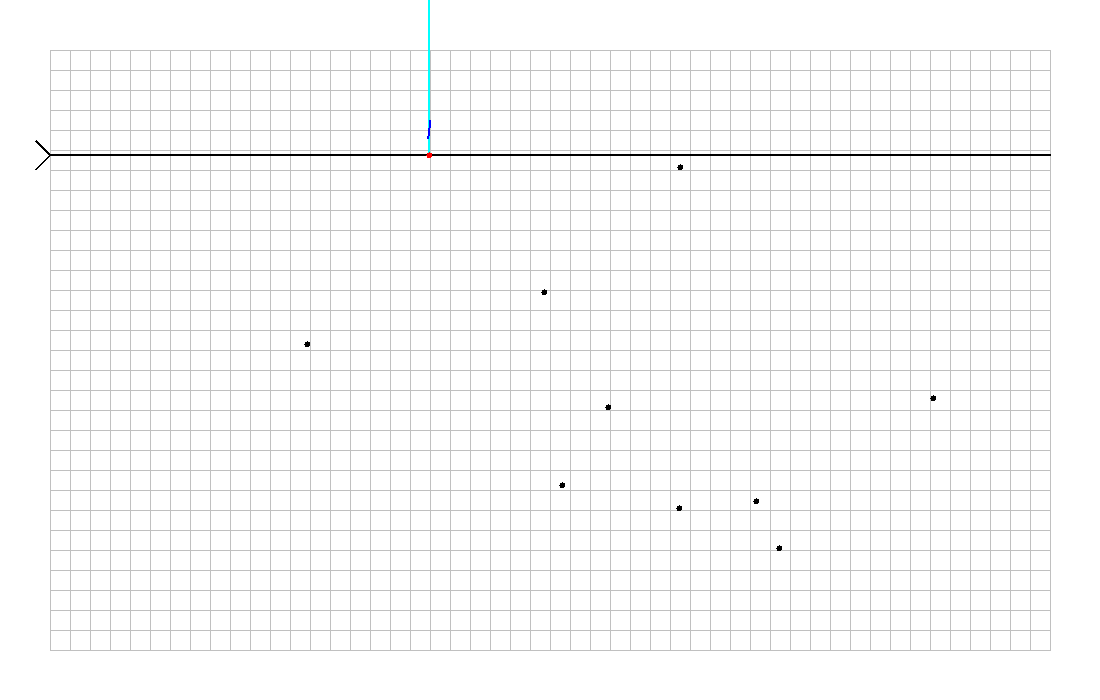
\includegraphics[width=0.6\linewidth]{capture_1-1}
}
\subfigure[Schritt 2]{
  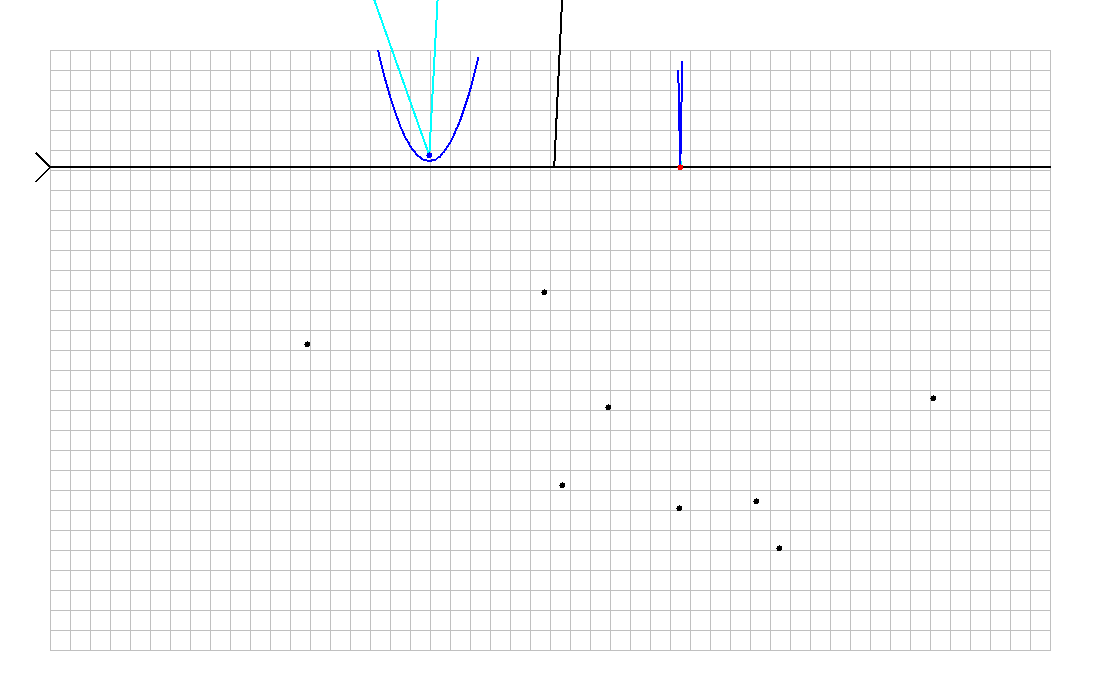
\includegraphics[width=0.6\linewidth]{capture_1-2}
}
\subfigure[Schritt 3]{
  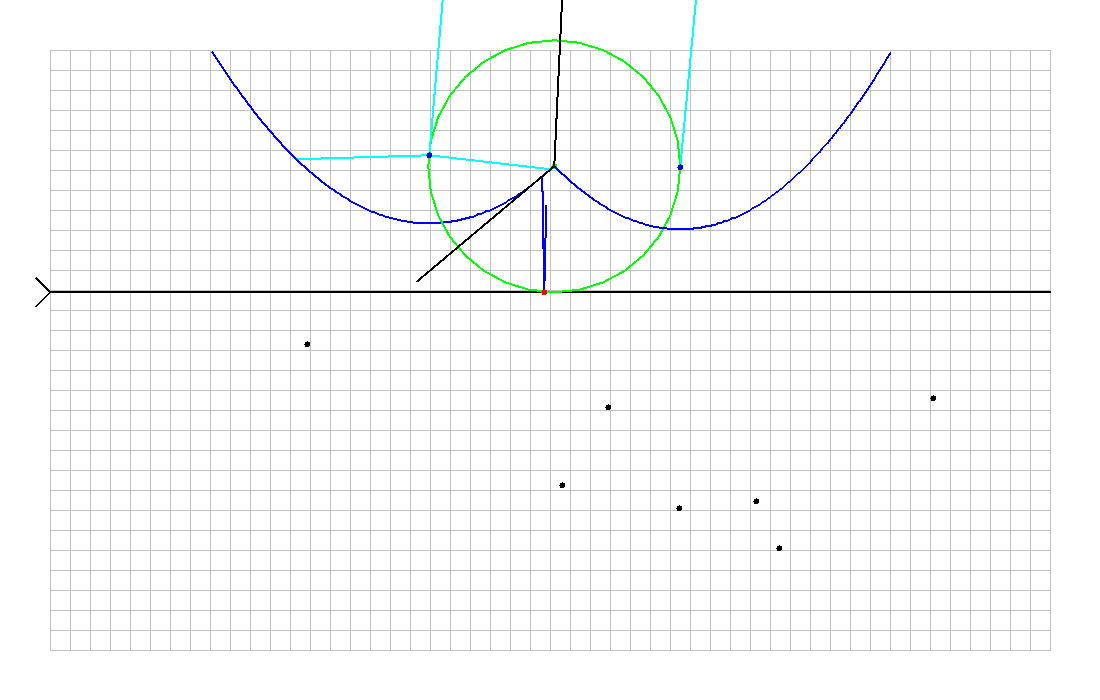
\includegraphics[width=0.6\linewidth]{capture_1-3}
}
\subfigure[Schritt 4]{
  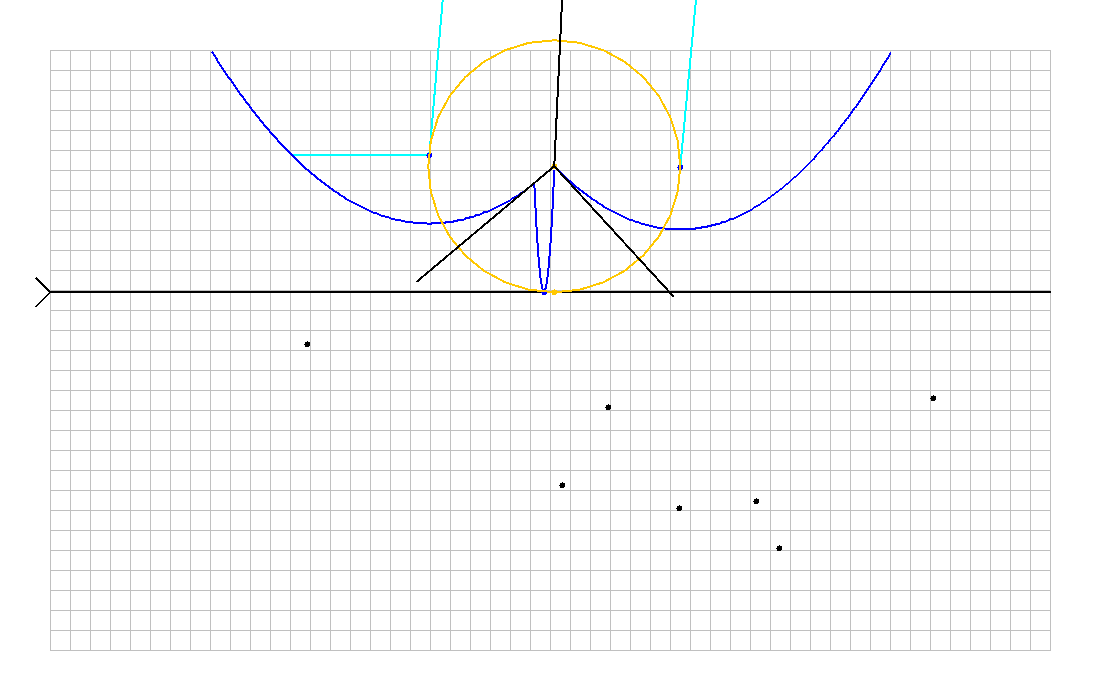
\includegraphics[width=0.6\linewidth]{capture_1-4}
}
\caption{Die ersten Schritte von Fortune's Sweep}
\label{fig:1-1}
\end{figure}

\begin{figure}[!htpb]
\centering
\subfigure[Schritt n-3]{
  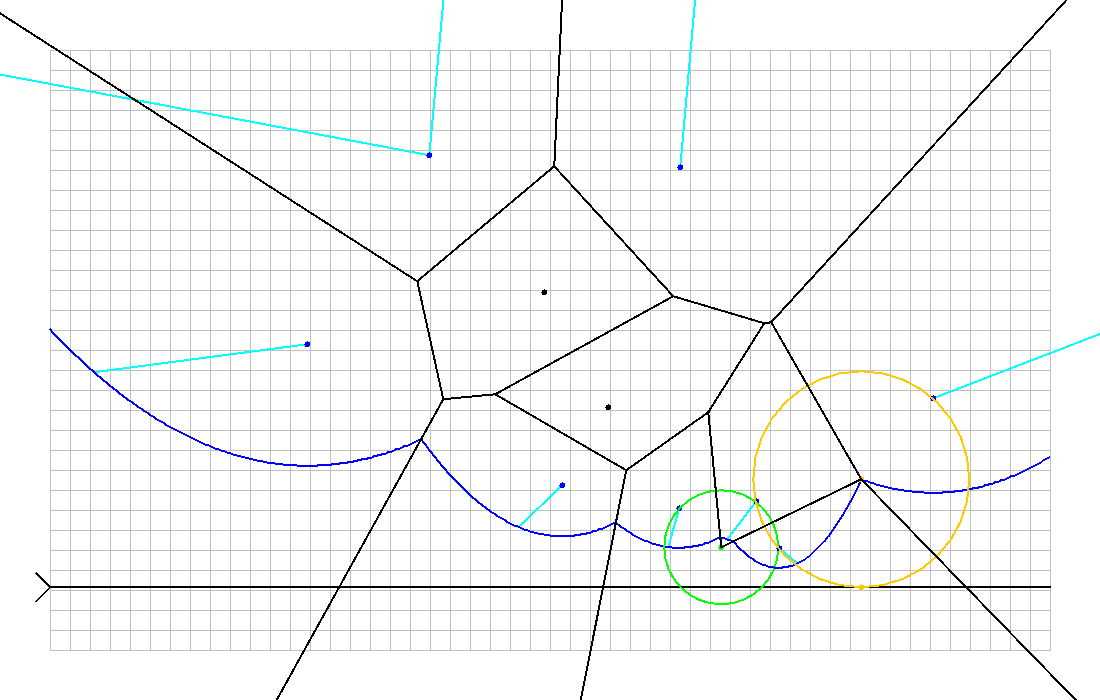
\includegraphics[width=0.6\linewidth]{capture_1-5}
}
\subfigure[Schritt n-2]{
  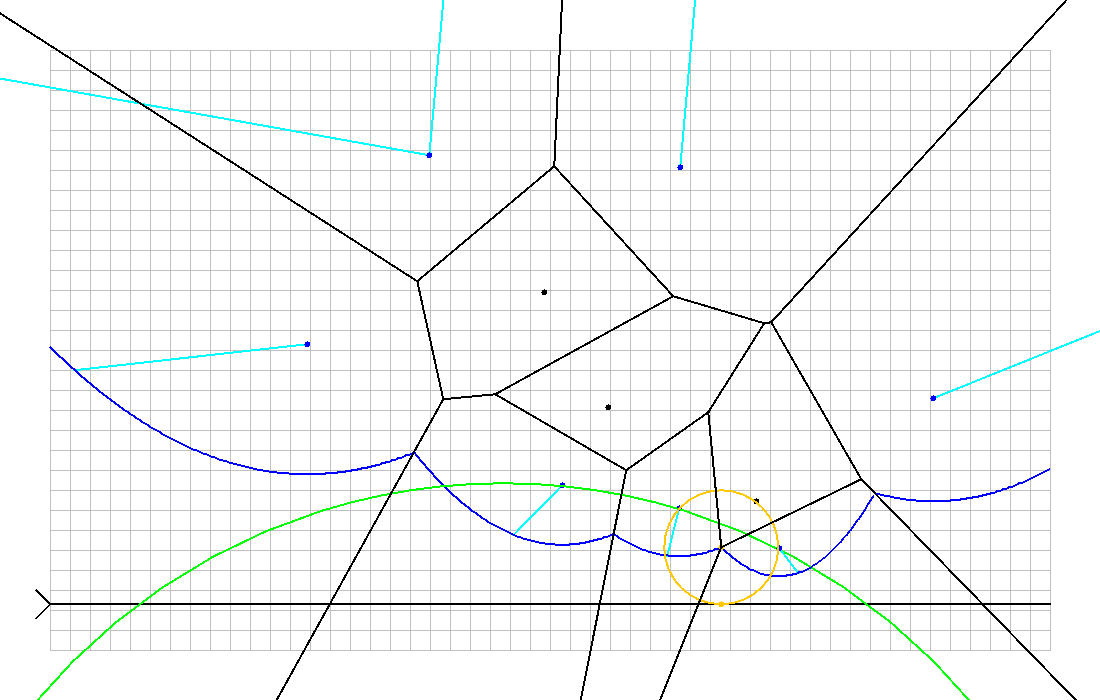
\includegraphics[width=0.6\linewidth]{capture_1-6}
}
\subfigure[Schritt n-1]{
  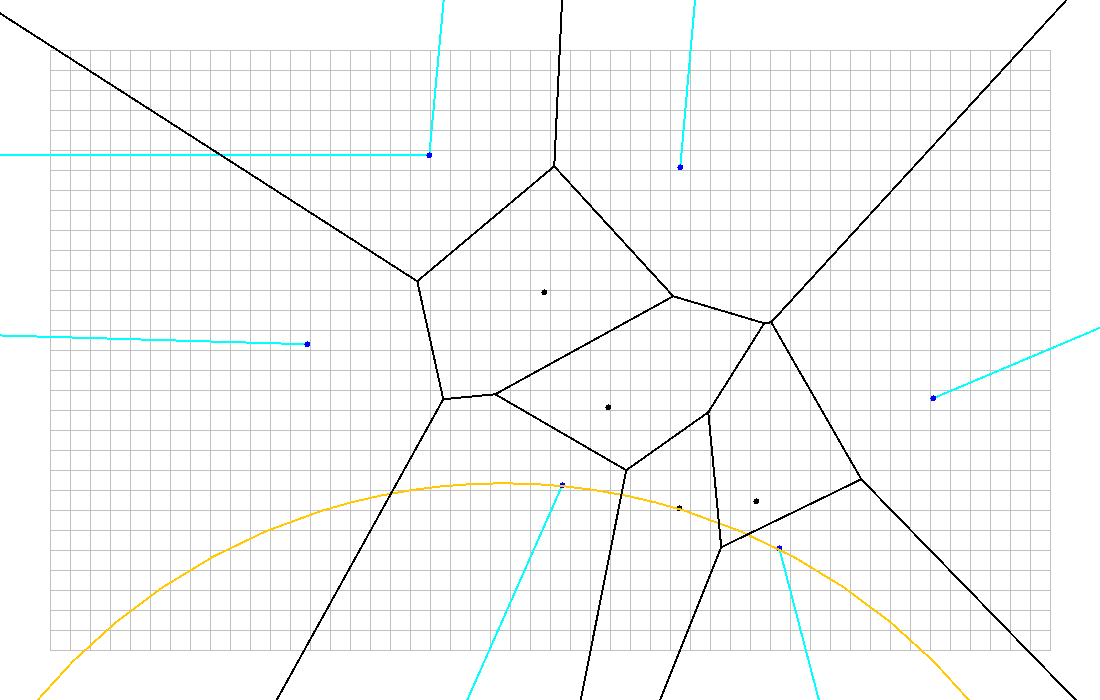
\includegraphics[width=0.6\linewidth]{capture_1-7}
}
\subfigure[Schritt n]{
  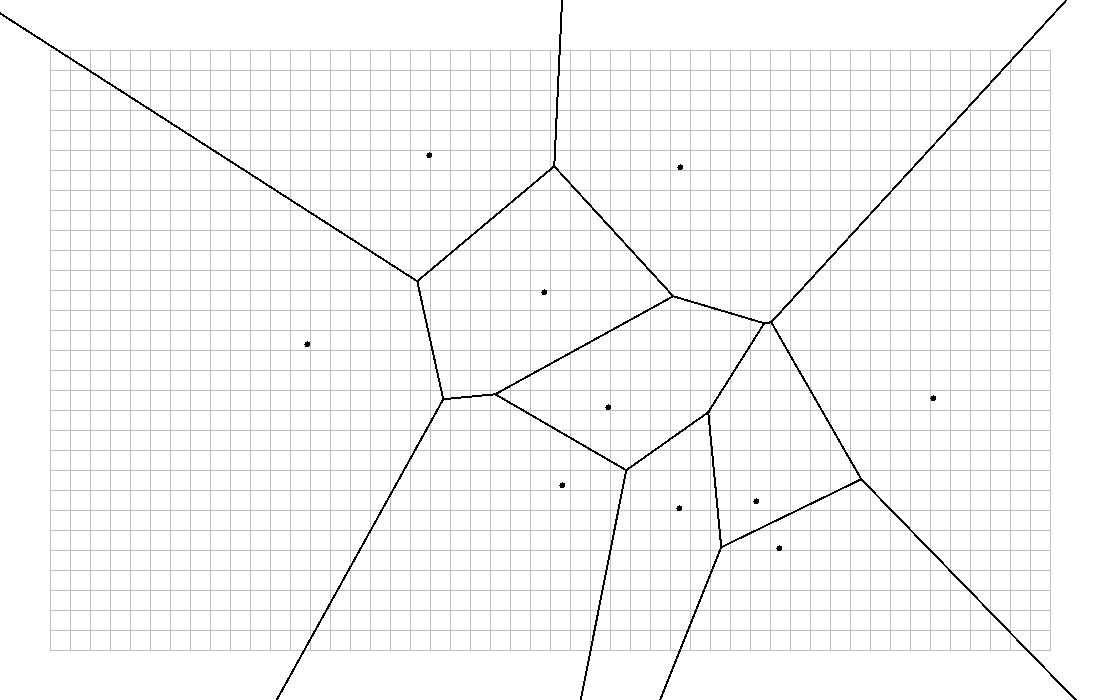
\includegraphics[width=0.6\linewidth]{capture_1-8}
}
\caption{Die letzten Schritte von Fortune's Sweep}
\label{fig:1-2}
\end{figure}
\end{task}

\newpage
\begin{task}{Potentialfelder}
\item[]
Potentialfelder sind eine sehr flexible Waffe im Kampf gegen die Wirren der Pfadfindung im zweidimensionalen Raum. In Ermangelung eines konkreten Anwendungsfalls implementieren wir sie völlig willkürlich und zwar wie folgt:

\begin{itemize}
\item Additive Felder können schwierig zu handeln sein (bspw. wenn ein Hinderniss nahe des Ziels dieses unerreichbar macht), unsere Felder sind deshalb exklusiv: an jedem Pixel wirkt nur die Kraft des einen Feldes, das dort am stärksten ist.
\item Alle attraktiven Felder haben im Zentrum den Wert $-1$ und alle repulsiven Felder den Wert $1$. Mit zunehmendem Abstand nähert sich die Stärke des Feldes dem Wert $0$ und zwar linear! Ein Feld $f$ ist somit eindeutig durch $f=(x,y,r)$ beschrieben, wobei $(x,y)$ das Zentrum des Feldes ist und $r$ der Abstand, bei dem unter Annahme einer linearen Abschwächung die Stärke des Feldes $0$ ist.
\item Um aus lokalen Optima zu entkommen, weisen wir bei der Pfadsuche einem besuchten Pixel eine zusätzlich repulsive Kraft zu.
\end{itemize}

Im Experiment werden jeweils 8 repulsive Felder erzeugt, mit zufälligen $x,y,r$. Umso roter ein Pixel visualisiert ist, desto stärker ist dort die repulsive Kraft.

Außerdem wird ein Zielpunkt (weiss) zufällig (im unteren, rechten Quadranten) erzeugt und mit einem attraktiven Feld versehen. Umso blauer ein Pixel, desto stärker ist dort die attraktive Kraft.

Der Startpunkt ist lila und liegt zufällig im oberen linken Quadranten. Der gefundene Weg zwischen Start und Ziel ist schwarz eingezeichnet.

Abbildung \ref{fig:2-1} zeigt vier Instanzen des Experiments. Vor allem in (c) ist schön zu sehen, wie aus einem lokalen Optimum ''entkommen'' wird.

\begin{figure}[!htpb]
\centering
\subfigure[]{
  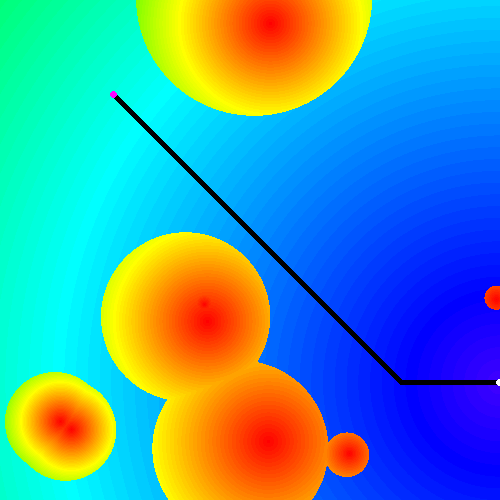
\includegraphics[width=0.48\linewidth]{../../src/u10/captures/capture_1-4}
}
\subfigure[]{
  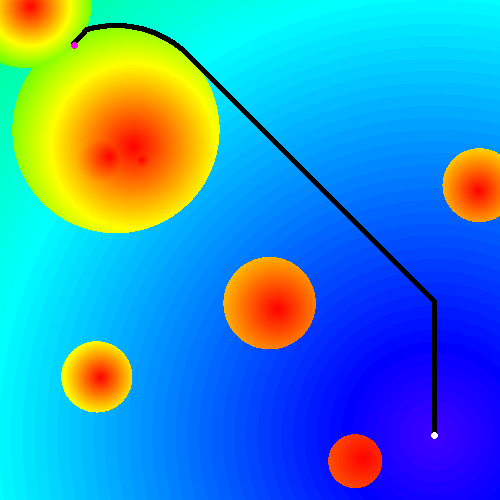
\includegraphics[width=0.48\linewidth]{../../src/u10/captures/capture_1-3}
}
\subfigure[]{
  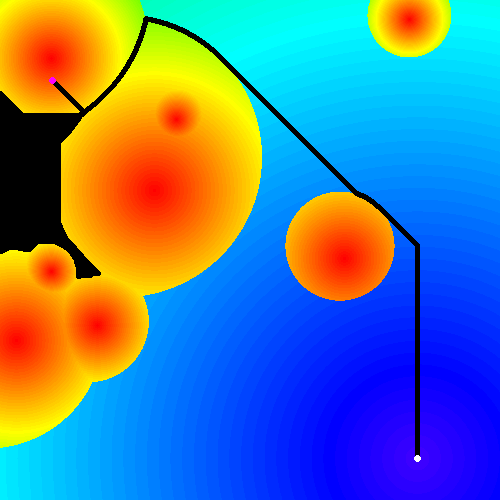
\includegraphics[width=0.48\linewidth]{../../src/u10/captures/capture_1-2}
}
\subfigure[]{
  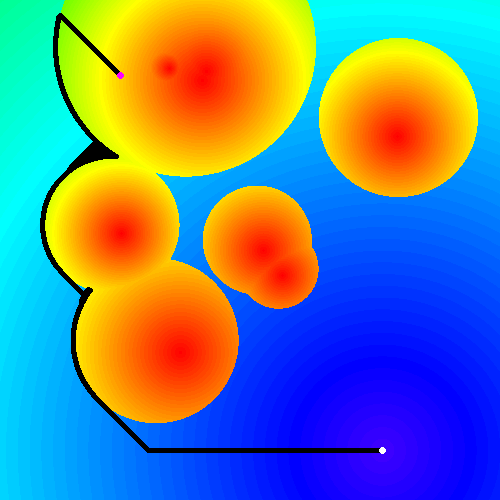
\includegraphics[width=0.48\linewidth]{../../src/u10/captures/capture_1-1}
}
\caption{Potentialfelder}
\label{fig:2-1}
\end{figure}
\end{task}
\end{document}